% This Source Code Form is subject to the terms of the Mozilla Public
% License, v. 2.0. If a copy of the MPL was not distributed with this
% file, You can obtain one at https://mozilla.org/MPL/2.0/.

\documentclass[a4paper, 12pt]{article}

\usepackage[english, russian]{babel}
\usepackage[T2A]{fontenc}
\usepackage[utf8]{inputenc}
\setlength{\parindent}{1cm}
\usepackage{graphicx}
\usepackage{amsmath}
\usepackage{amssymb}
\usepackage{amsfonts}
\usepackage{array}
\usepackage{booktabs}
\usepackage{wrapfig}
\usepackage{caption} %заголовки плавающих объектов
\captionsetup[table]{justification=centering} %установки для заголовков таблиц
\captionsetup[figure]{justification=centering} %установки для заголовков таблиц

\begin{document}

\begin{center}
	\subsubsection*{Отчёт к лабораторной работе №22}
	
	\subsubsection*{"Исследование инвертирующего усилителя"}
	
	\subsubsection*{Преподаватель: Петриков В. Д.}
	
	Выполнил студент третьего курса вышей школы фундаментальных физический исследований: Куликовских Илья
	
	Группа: 5030302/30801
\end{center}

\subsubsection*{Исследование инвертирующего усилителя: снятие передаточной характеристики, наблюдение нелинейных искажений}

Был собран инвертирующий усилитель (ИУ) с резисторами \( R_\alpha = 5.1 \, \text{кОм} \) и \( R_\beta = 10 \, \text{кОм} \) в цепи обратной связи (рис. 1). Режим питания ОУ – двуполярный: \( \pm 15 \, \text{В} \). К входу подключен генератор синусоидального напряжения. Частота входного напряжения 1 кГц.

\begin{figure}[htpb]
	\centering
	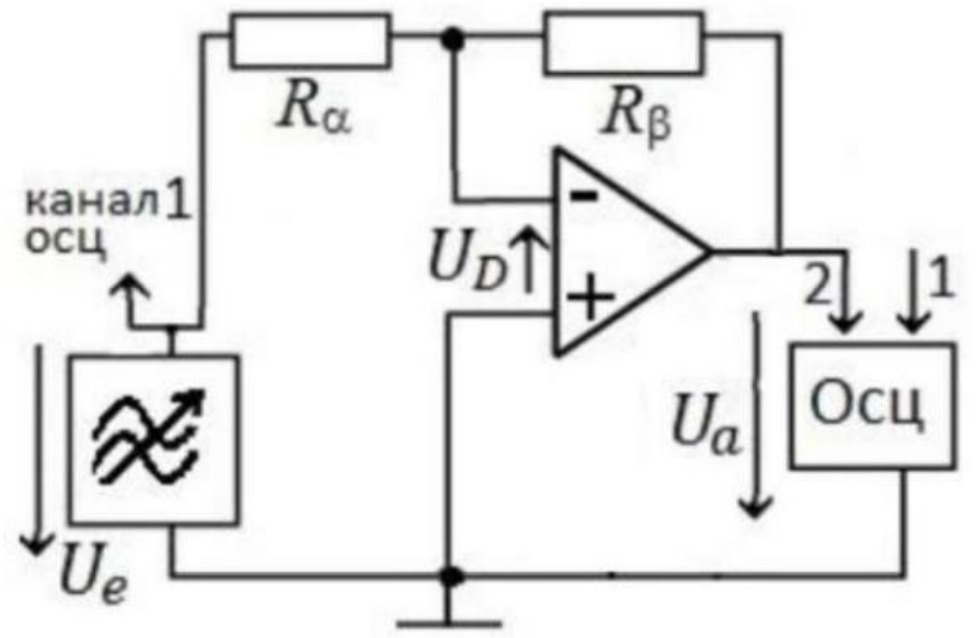
\includegraphics[width=0.5\textwidth]{22-1.png}
	\caption{Схема исследования ИУ}
\end{figure}

Характеристики устройств:
\[ R_\alpha = 5.1 \, \text{кОм} \]
\[ R_\beta = 10 \, \text{кОм} \]

Получена следующая передаточная характеристика ИУ \( U_a(U_e) \) в диапазоне входного напряжения, включающего области усиления и ограничения напряжения на выходе ОУ (рис. 2).

\begin{figure}[htpb]
	\centering
	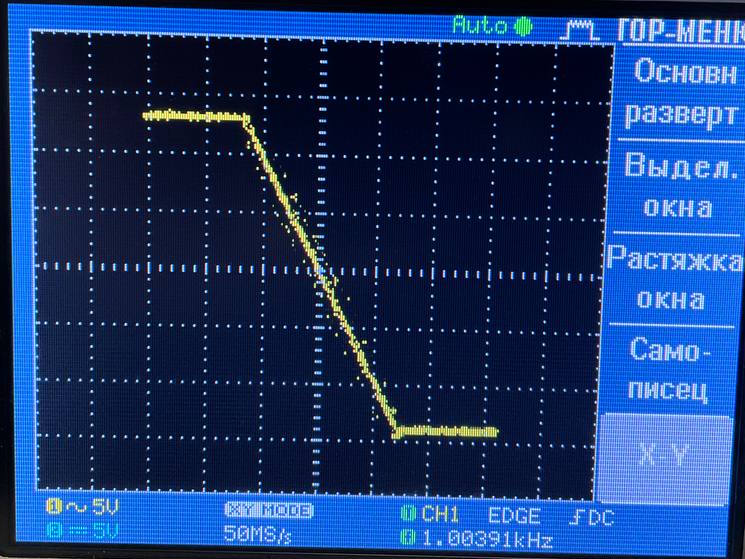
\includegraphics[width=0.5\textwidth]{22-2.jpg}
	\caption{Кривая $U_a$ ($U_e$)}
\end{figure} 

Значения коэффициента усиления ИУ и границ области усиления:

Коэффициент усиления как отношение величины по оси ординат к величине по оси абсцисс:
\[ K = \dfrac{U_a}{U_e} = \dfrac{10}{-5} = -2 \]

Границы выходного напряжения через диапазон по оси ординат, где график – линейный: от \( -14 \, \text{В} \) до \( 14 \, \text{В} \).
Границы области усиления через диапазон по оси абсцисс, где график – линейный: от \( -6 \, \text{В} \) до \( 6 \, \text{В} \).

После перевода осциллографа в режим линейной развёртки при выходе за пределы области усиления получились следующие осциллограммы входного и искажённого выходного напряжений (рис. 3).

\begin{figure}[htpb]
	\centering
	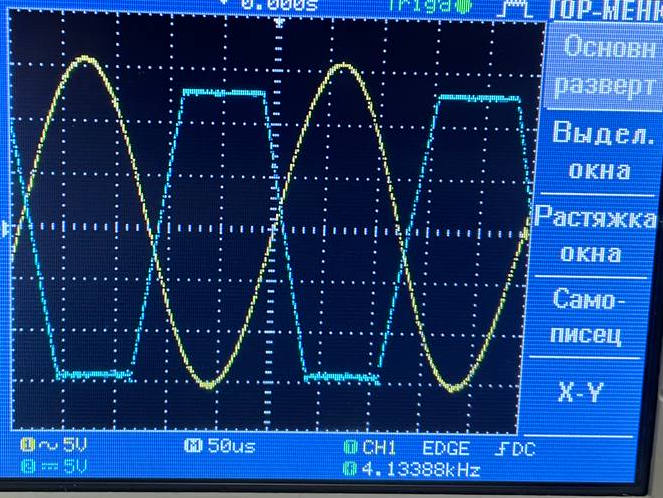
\includegraphics[width=0.5\textwidth]{22-3.jpg}
	\caption{Низкочастотные искажения на выходе ОУ}
\end{figure} 

К первому (жёлтому) каналу подключено входное напряжение, ко второму (синему) – выходное. Для обоих напряжений масштаб по оси ординат одинаковый и равен \( 5 \, \text{В} \).

После уменьшения интенсивности входного напряжения до исчезновения искажения и дальнейшего увеличении частоты сигнала мы вошли в область высокочастотных динамических искажений и получили следующую осциллограмму (рис. 4).

\begin{figure}[htpb]
	\centering
	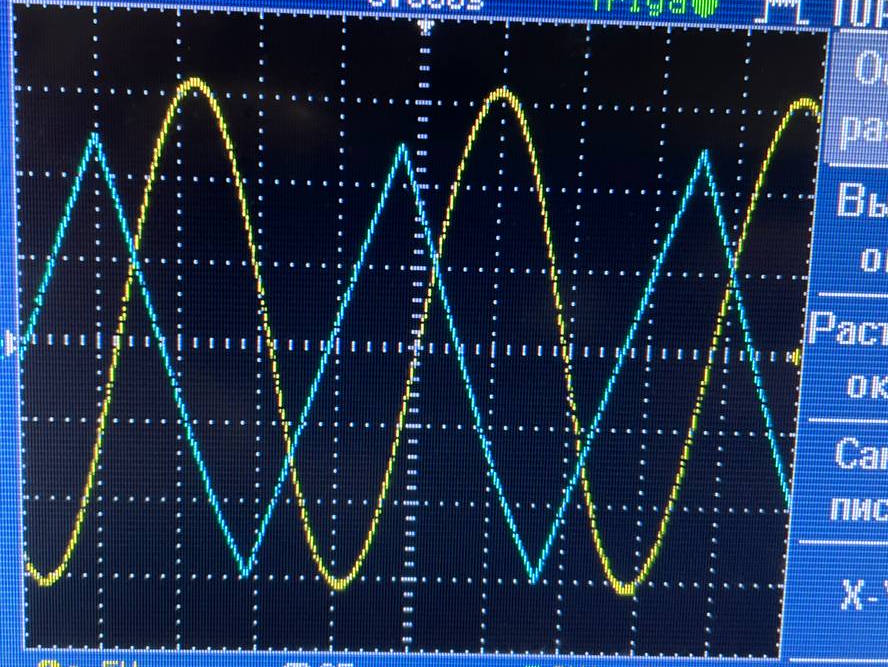
\includegraphics[width=0.5\textwidth]{22-4.jpg}
	\caption{Динамические искажения на выходе ОУ}
\end{figure} 

Оценка максимальной скорости нарастания выходного напряжения \( V \):

Плавно уменьшили амплитуду внешнего воздействия до амплитуды выходного напряжения \( U_{am} \), при которой форма осциллограммы подобна синусоиде (рис. 5).

\begin{figure}[htpb]
	\centering
	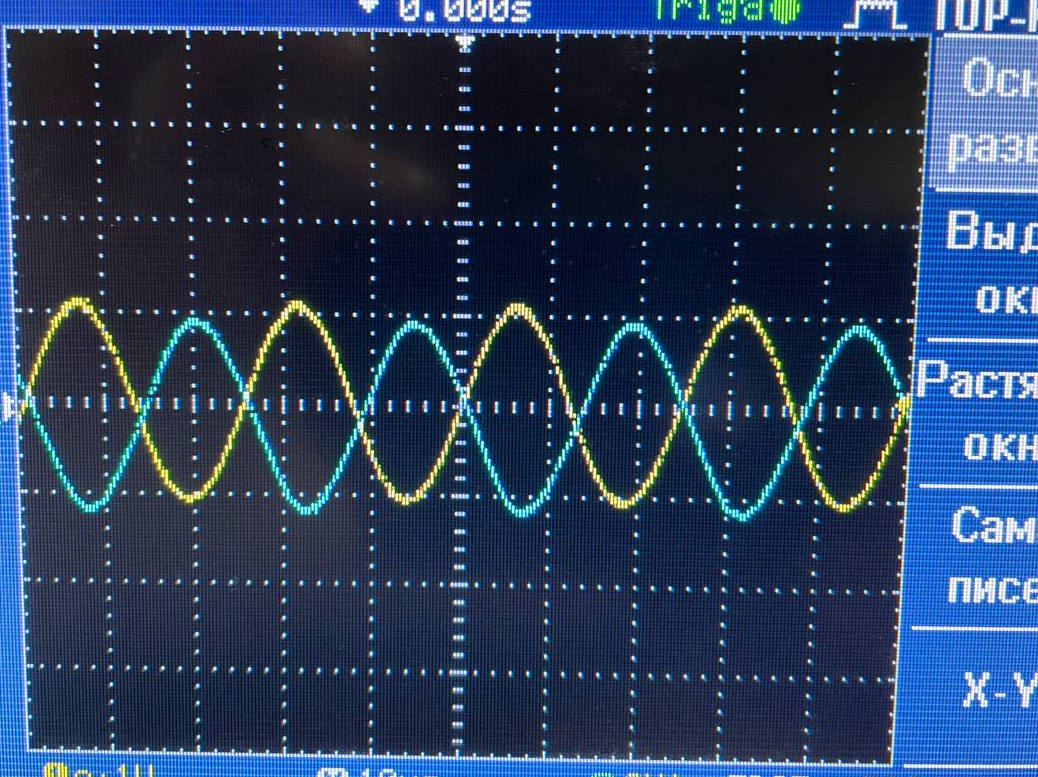
\includegraphics[width=0.5\textwidth]{22-5.jpg}
	\caption{Осциллограмма входного и выходного напряжений}
\end{figure} 

Полученные значения амплитуды выходного напряжения \( U_{am} = 0.5 \, \text{В} \) и частоты синусоиды \( f = 100 \, \text{кГц} \) подставим в формулу для оценки максимальной скорости нарастания:
\[ V = 2\pi fU_{am} = 0.3 \times 10^6 \, \text{В/мкс} \]

Сравнив с данными справочника, можно сделать вывод, что в данной лабораторной работе использовался ОУ К153УД2, у которого максимальная скорость нарастания \( > 0.5 \, \text{В/мкс} \).


\subsubsection*{Вывод}

В лабораторной работе использовался ОУ К153УД2, это видно после сравнения полученных результатов с данными из справочника.

При высоких частотах (100 кГц) и большой амплитуде выходной сигнал искажается из-за ограниченной скорости нарастания ОУ. Это означает что данный ОУ не подходит для использования в системах с высокочастотными сигналами, например в радиочастотных системах (Wi-Fi, Bluetooth).

Из полученных АЧХ видно, что в зависимости от схемы на промежутке до 10–100 кГц ОУ выдаёт стабильное усиление. Также для неинвертирующего ОУ коэффициент усиления примерно до 40 дБ. Его можно применять в аудиоусилителях, в различных датчиках с медленными сигналами, требующими точности (датчики температур, давления и т.п.). При этом для усиления на конкретных частотах можно использовать несколько усилителей. Например, для усиления в 1000 раз на частоте 100 кГц необходимо использовать 3 усилителя.

Из-за возможности суммирования сигналов ОУ можно применять в различных схемах, где это необходимо, например в ЦАП и АЦП схемах.

ОУ хорошо справляется с усилением слабых сигналов, фильтрацией и обработкой низкочастотных сигналов, и точными аналоговыми вычислениями (суммированием). То есть его можно использовать для аудио, в измерительных приборах и системах управления. Для радиочастот или цифровых интерфейсов данный ОУ не подходит.

\end{document}